\newpage
\section{Durchführung}
\label{sec:Durchführung}
\begin{figure}
	\label{fig:platine}
	\centering
	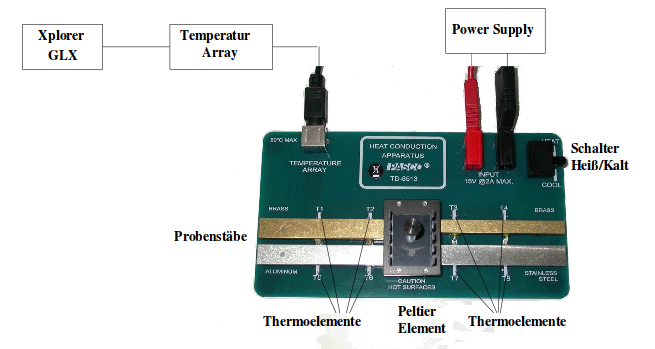
\includegraphics[width=\textwidth]{Bilder/Aufbau.png}
	\caption{Aufbau der Platine}
\end{figure}

Um den zeitlichen Temperaturverlauf von vier Metallproben bestimmen zu können, wurden diese auf der in Abbildung 1 gezeigten Platine angebracht. Mit dem mittig aufgesetzten \emph{Peltier-Element}, bestehend aus zwei Halbleitern unterschiedlicher Energieniveaus, können die Stäbe durch ausnutzen des Peltier-Effekts simultan geheizt oder gekühlt werden. Betrieben wird das Element durch eine angeschlossene \emph{Spannungsquelle}. 
An jedem Stab befinden sich zwei \emph{Thermoelemente}, bestehend aus zwei metallischen Leitern, die an den Orten $x_1$ und $x_2$ die Temperaturen der Stäbe aufzeichnen. Dabei ruft die Temperaturdifferenz - gegensätzlich zum Peltier-Element - einen Spannungsunterschied hervor, der gemessen wird. Diese Daten werden über ein \emph{Teperature-Array} an den \emph{GLX-Datenlogger} weitergegeben, dort aufgezeichnet und auf einen USB-Stick exportiert. 

Vor Messbeginn werden sowohl die korrekte Verkabelung, als auch die Einstellungen des Datenloggers überprüft; alle acht Thermoelemente $T_\mathup{1}$-$T_\mathup{8}$ sollten eine Temperatur aufzeichnen.

\subsection{Statische Messung}

Das Peltier-Element wird mit einer Spannung $U_\mathup{P}=5 \si{\volt}$ bei maximalem Strom $I$ betrieben. Im Datenlogger wird eine Abtastrate von $\Delta{t}=5\si{\second}$ eingestellt. Nachdem die Isolierung auf die Probestäbe gelegt wurde, um einen Wärmeaustausch mit der Umgebung zu vermeiden, und der Schalter umgelegt ist beginnt das Peltier-Element zu heizen. Der Datenlogger zeichnet alle 5 Sekunden die Temperaturen $T_i, i=1,..,8$ der Thermoelemente auf bis Thermoelement 7 eine Temperatur von $T_\mathup{7}\approx 43°C$ anzeigt. Anschließend werden die Isolierungen abgenommen, das Peltier-Element auf "cool" gestellt, die aufgenommenen Daten zur Auswertung auf einen USB-Stick übertragen und die für die Auswertung benötigten Diagramme des Temperaturverlaufs ausgedruckt.

\subsection{Dynamische Messung}
Nachdem die Stäbe wieder auf eine Temperatur von $T<30°C$ gekühlt wurden, werden die Isolierungen erneut aufgelegt und das Peltier-Element beginnt bei einer Spannung von $U_\mathup{P}=8 \si{\volt}$ zu heizen. Die Thermoelemente zeichnen nun mit $\Delta{t}=2\si{\second}$ den Temperaturverlauf auf.

Nach $\tilde{t}=40\si\second$ wird das Peltier-Element umgeschaltet und die Stäbe für weitere 40 s gekühlt. Dieser Vorgang wird wiederholt, bis zehn Perioden von $T=80\si\second$ Dauer aufgezeichnet wurden. Anschließend werden die Stäbe analog zur statischen Messung wieder heruntergekühlt. Schließlich wird die dynamsiche Methode noch einmal wiederholt, wobei die Periodendauer nun $T=200\si\second$ beträgt. Erneut werden die Messdaten auf einen USB-Stick übertragen und einige Temperaturverläufe graphisch dargestellt und ausgedruckt.
